We explore three different adaptation strategies for mesh adaptation based on the VMS-based estimated error. 

\subsection{Zonal Adaptation}

%TODO: Coarsening can possibly be done but was not needed in this work
%TODO: Maybe show some schematics. Cylinder/airfoil flow. Simple schematics with 2/3 zones. 
%TODO: Change zonal/refinement adaptation to zonal adaptation



The first strategy we employ is error estimator based zonal refinement/adaptation. 
In this strategy, we obtain an initial solution on a baseline mesh for the problem at hand. The VMS-based error estimator is then applied to the solution corresponding to this mesh, and based on the estimated error, the mesh is refined by a factor of 2 in particular zones where high error values are found. Estimated error for this adapted mesh is then calculated, and the mesh is again refined by a factor of 2 in zones of high error. This process is repeated till it is computationally feasible, or a convergence is reached.

This strategy is represented in Figure \ref{fig:zonal_based_strat}

\begin{figure}[H]
	\centering
	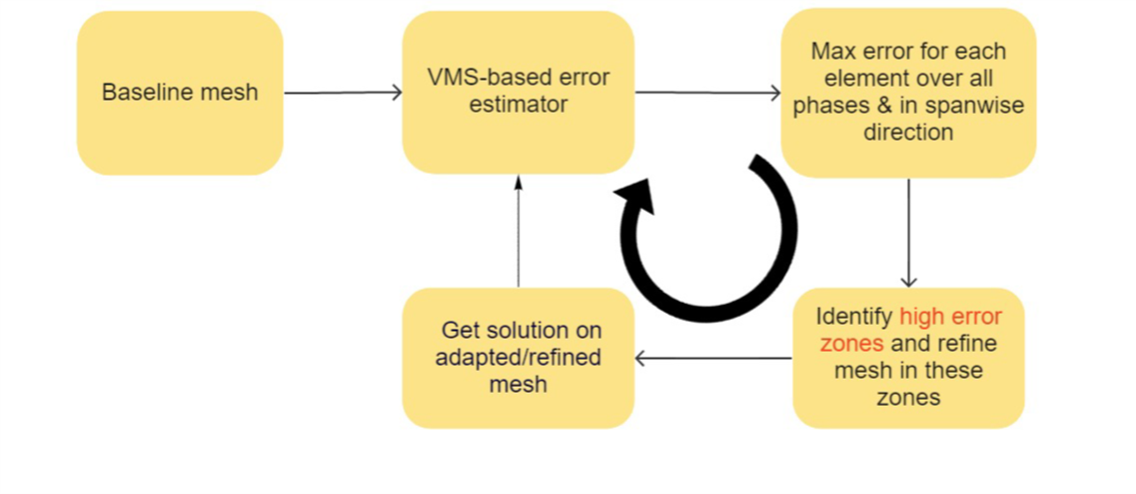
\includegraphics[width=1\textwidth]{figures/adapt_strat/zonal_based.png}
	\caption{Zonal Refinement/Adaptation Strategy}
	\label{fig:zonal_based_strat}
\end{figure}

\subsection{Nodal Size Field-based Adaptation}

The second strategy we employ is fully automated mesh adaptation based on the VMS-based error estimator. In this strategy, the estimated error and a specified target error are used to compute the desired mesh size or resolution in a local fashion, i.e., at every mesh vertex. We refer to this as the nodal size field, and the mesh is refined or coarsened based on this nodal size field. 

In this adaptive strategy, the VMS-based error is calculated on the initial mesh. Based on the estimated error, a nodal size field is calculated using the following equation \cite{zhang19}

\begin{equation}
	\frac{e_k}{\tilde{e}_k} = \left(\frac{h_{old}}{h_{new}}\right)^{m+N/2} 
	\label{eq:diez}
\end{equation}

Here, $e_k$ is the measured local error (in the $\HOne$-seminorm) at an element $k$, $\tilde{e}_k$ is the target error for an element specified by the user, $m$ is the polynomial order of the approximation space (i.e., $m=1$ for the linear finite elements used currently) , and $N$ is the number of spatial dimensions. $h_{old}$ is current size of the element, and $h_{new}$ is the desired new mesh size.
This new mesh size at the element level is assembled at the node/vertex level to perform mesh adaptation.
This strategy is represented in Figure \ref{fig:size_based_strat}.

\begin{figure}[H]
	\centering
	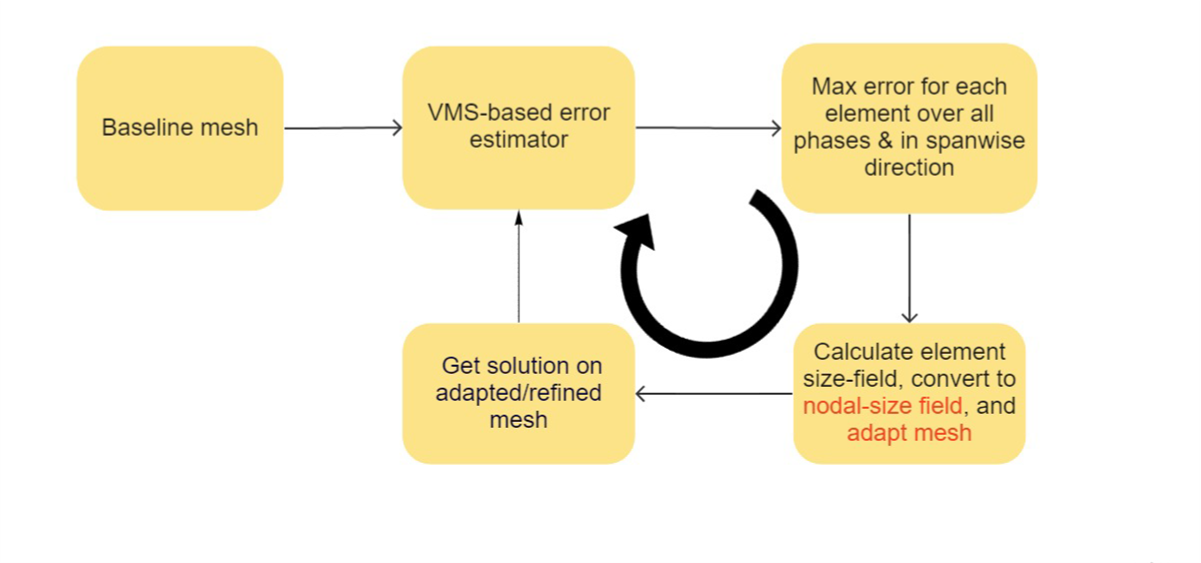
\includegraphics[width=1\textwidth]{figures/adapt_strat/size_based.png}
	\caption{Nodal Size Field-based Refinement/Adaptation Strategy}
	\label{fig:size_based_strat}
\end{figure}

\subsection{Feature-based Refinement/Adaptation}

The third strategy is to employ feature-based refinement/adaptation. 
One of the primary flow features is the leading edge vortex (LEV) in the current problems of interest focused on surging airfoils. LEV forms during the retreating portion of the surging cycle when the boundary layer rolls up, separates from the airfoil, and advects away from the airfoil.
This allows for refinement around the dominant flow features and also along the path/trajectory of such features, in particular for LEV.


\subsubsection{LEV Detection and Tracking}

%TODO: Show pics and schematics from AIAA paper and presentations (LEV trace)

In this section, we quantify the evolution of the LEV based on its size and position.
In order to do so, for each case at first the phase of formation of the LEV is detected and in subsequent phases the LEV is tracked.
Pressure and velocity data is analyzed to automatically detect the formation of the LEV.
In the retreating portion of the cycle, location with minimum pressure is determined starting at $\psi=180^\circ$.
The first phase at which the minimum pressure location is off the airfoil surface (i.e., away from the airfoil and into the flow) is tagged to be a potential phase for LEV formation.
At this potential phase, velocity profile is obtained over multiple lines passing through the minimum pressure location.
These are radial lines that are taken at an equispaced interval along the azimuth in the plane of the airfoil (note that the data is averaged in the spanwise direction).
Along these lines, at first a relative velocity is computed with respect to the velocity at the minimum pressure location.
Subsequently, normal component of the relative velocity is obtained (i.e., normal to each line), which is the azimuthal or tangential component in the polar coordinate system centered around the minimum pressure location.
The azimuthal component (of the relative velocity) is analyzed against the velocity profile of a Lamb-Oseen vortex.
It is noteworthy that the azimuthal component of the relative velocity along several radial lines at multiple phases in the surging cycle were visually analyzed for different cases and found to fit the Lamb-Oseen vortex model fairly well.

\subsubsection{LEV-based Refinement/Adaptation}

%TODO: Check numbering in a running text for a numbered list

For a given simulation, we can follow three steps: 1) get information on the approximate path and extent that a certain feature will follow, 2) estimate the error along this path/region, and 3) perform refinement/adaptation along this path.
For example, in the case of flow over surging airfoils, the path and size of LEV over a surging cycle is used to detect portions in the mesh where refinement is applied.
Similarly, other features such as trailing edge vortex (TEV) can also be targeted using such a feature-based refinement.

%TODO: Schematic to illustrate feature-based adaptation zone
%TODO: Flowchart

This strategy is represented in Figure \ref{fig:feature_based_strat}.

\begin{figure}[H]
	\centering
	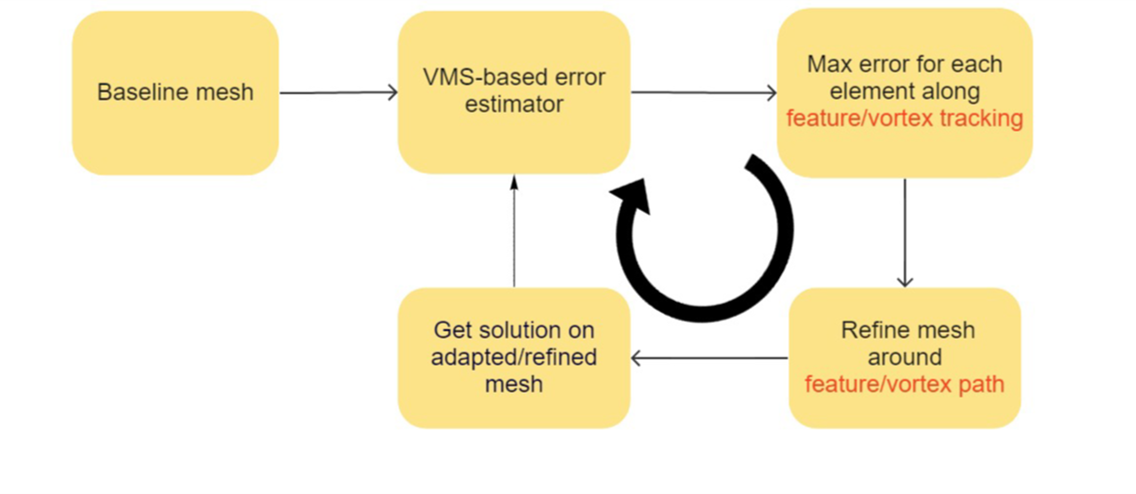
\includegraphics[width=1\textwidth]{figures/adapt_strat/feature_based.png}
	\caption{Feature-based Refinement/Adaptation Strategy}
	\label{fig:feature_based_strat}
\end{figure}


